% Options for packages loaded elsewhere
\PassOptionsToPackage{unicode}{hyperref}
\PassOptionsToPackage{hyphens}{url}
%
\documentclass[
]{article}
\usepackage{amsmath,amssymb}
\usepackage{lmodern}
\usepackage{iftex}
\ifPDFTeX
  \usepackage[T1]{fontenc}
  \usepackage[utf8]{inputenc}
  \usepackage{textcomp} % provide euro and other symbols
\else % if luatex or xetex
  \usepackage{unicode-math}
  \defaultfontfeatures{Scale=MatchLowercase}
  \defaultfontfeatures[\rmfamily]{Ligatures=TeX,Scale=1}
\fi
% Use upquote if available, for straight quotes in verbatim environments
\IfFileExists{upquote.sty}{\usepackage{upquote}}{}
\IfFileExists{microtype.sty}{% use microtype if available
  \usepackage[]{microtype}
  \UseMicrotypeSet[protrusion]{basicmath} % disable protrusion for tt fonts
}{}
\makeatletter
\@ifundefined{KOMAClassName}{% if non-KOMA class
  \IfFileExists{parskip.sty}{%
    \usepackage{parskip}
  }{% else
    \setlength{\parindent}{0pt}
    \setlength{\parskip}{6pt plus 2pt minus 1pt}}
}{% if KOMA class
  \KOMAoptions{parskip=half}}
\makeatother
\usepackage{xcolor}
\IfFileExists{xurl.sty}{\usepackage{xurl}}{} % add URL line breaks if available
\IfFileExists{bookmark.sty}{\usepackage{bookmark}}{\usepackage{hyperref}}
\hypersetup{
  pdftitle={Test2},
  pdfauthor={Paul Christmann},
  hidelinks,
  pdfcreator={LaTeX via pandoc}}
\urlstyle{same} % disable monospaced font for URLs
\usepackage[left=1.5cm,right=1.5cm,top=1.5cm,bottom=1.5cm]{geometry}
\usepackage{graphicx}
\makeatletter
\def\maxwidth{\ifdim\Gin@nat@width>\linewidth\linewidth\else\Gin@nat@width\fi}
\def\maxheight{\ifdim\Gin@nat@height>\textheight\textheight\else\Gin@nat@height\fi}
\makeatother
% Scale images if necessary, so that they will not overflow the page
% margins by default, and it is still possible to overwrite the defaults
% using explicit options in \includegraphics[width, height, ...]{}
\setkeys{Gin}{width=\maxwidth,height=\maxheight,keepaspectratio}
% Set default figure placement to htbp
\makeatletter
\def\fps@figure{htbp}
\makeatother
\setlength{\emergencystretch}{3em} % prevent overfull lines
\providecommand{\tightlist}{%
  \setlength{\itemsep}{0pt}\setlength{\parskip}{0pt}}
\setcounter{secnumdepth}{-\maxdimen} % remove section numbering
\usepackage[font={small,it}, labelfont={bf}]{caption}
\usepackage{amsmath}
\usepackage{booktabs}
\usepackage{caption}
\usepackage{longtable}
\ifLuaTeX
  \usepackage{selnolig}  % disable illegal ligatures
\fi

\title{Test2}
\author{Paul Christmann}
\date{2022-07-12}

\begin{document}
\maketitle

\hypertarget{the-expression-of-all-tras-associated-with-a-tissue-cannot-be-used-to-infer-organ-development}{%
\subsubsection{The expression of all TRAs associated with a tissue
cannot be used to infer organ
development}\label{the-expression-of-all-tras-associated-with-a-tissue-cannot-be-used-to-infer-organ-development}}

In this research, we attempt to draw conclusions about the developmental
state of a tissue based on the expression of genes associated with it
alone. Therefore, we analyzed the share of differentially expressed
transcripts above a certain expression level over time, as shown in Fig.
???A. Furthermore, we observed trends within the median expression of
all differentially expressed transcripts associated with a tissue (Fig.
???B). Since both metrics only showed in miniscule changes, we
hypothesized that distinct, counteracting trends in expression exsisted
within one tissue. Thus, k-means clustering was used to determine groups
of TRAs with similar expression patterns. For each of these clusters,
the median expression was plotted as shown in Fig. ???C.

\begin{figure}
\centering
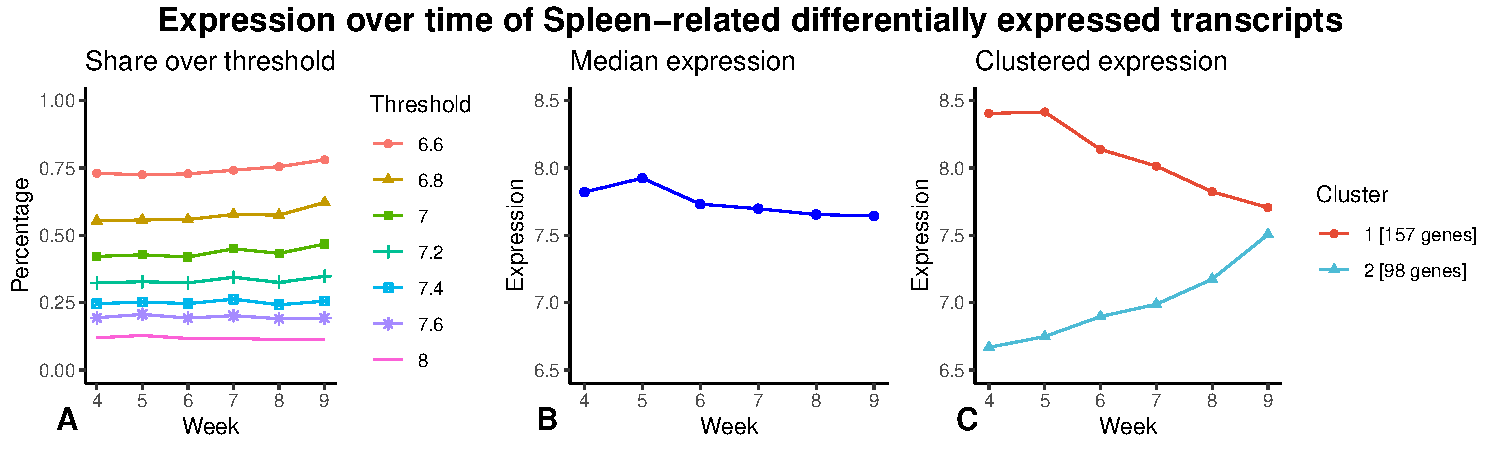
\includegraphics{Test2_files/figure-latex/unnamed-chunk-5-1.pdf}
\caption{A. For different expression thresholds the share of
differentially expressed transcripts with higher expressions than the
threshold is depicted. B. The median}
\end{figure}

\begin{figure}
\centering
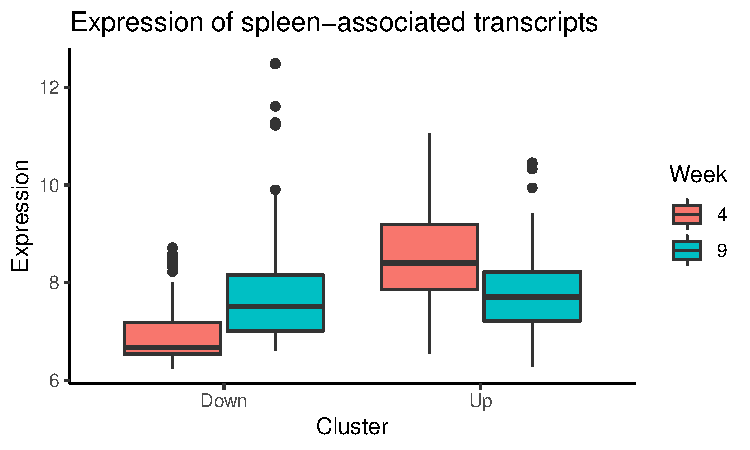
\includegraphics{Test2_files/figure-latex/unnamed-chunk-10-1.pdf}
\caption{A further look on the expression of transcripts in the up- and
downregulated clusters shows that the upregulated transcripts are close
to the minimum expression level between 6 and 7 in week 4 and showing
expressions between 7 and 8.5 by week 9. In contrast, the downregulated
genes have very high expression levels (8-9) by week 4 and decrease to a
more moderate expression between 7 and 8.5 analogous to the upregulated
transcripts.}
\end{figure}

\captionsetup[table]{labelformat=empty,skip=1pt}
\begin{longtable}{llllc}
\caption*{
{\large Spleen - Downregulated} \\ 
{\small List of differentially epxressed genes}
} \\ 
\toprule
Transcript & Gene & Protein & Summary & Expression\_over\_time \\ 
\midrule
ENST00000251296 & IGSF21 & immunoglobin superfamily member 21 & Component of  the centromere & <?xml version='1.0' encoding='UTF-8' ?><svg xmlns='http://www.w3.org/2000/svg' xmlns:xlink='http://www.w3.org/1999/xlink' class='svglite' width='85.04pt' height='14.17pt' viewBox='0 0 85.04 14.17'><defs>  <style type='text/css'><![CDATA[    .svglite line, .svglite polyline, .svglite polygon, .svglite path, .svglite rect, .svglite circle {      fill: none;      stroke: #000000;      stroke-linecap: round;      stroke-linejoin: round;      stroke-miterlimit: 10.00;    }    .svglite text {      white-space: pre;    }  ]]></style></defs><rect width='100%' height='100%' style='stroke: none; fill: none;'/><defs>  <clipPath id='cpMC4wMHw4NS4wNHwwLjAwfDE0LjE3'>    <rect x='0.00' y='0.00' width='85.04' height='14.17' />  </clipPath></defs><g clip-path='url(#cpMC4wMHw4NS4wNHwwLjAwfDE0LjE3)'><polygon points='11.86,12.55 22.53,11.69 33.19,12.52 43.85,12.27 54.52,8.60 65.18,1.63 65.18,244.58 54.52,244.58 43.85,244.58 33.19,244.58 22.53,244.58 11.86,244.58 ' style='stroke-width: 0.00; stroke: none; fill: #D3D3D3; fill-opacity: 0.75;' /><polyline points='11.86,12.55 22.53,11.69 33.19,12.52 43.85,12.27 54.52,8.60 65.18,1.63 ' style='stroke-width: 1.07; stroke: none;' /><text x='68.38' y='3.25' style='font-size: 5.69px; font-family: "Arial";' textLength='10.24px' lengthAdjust='spacingAndGlyphs'>6.9</text><polyline points='11.86,12.55 22.53,11.69 33.19,12.52 43.85,12.27 54.52,8.60 65.18,1.63 ' style='stroke-width: 1.07; stroke-linecap: butt;' /><circle cx='65.18' cy='1.63' r='0.89' style='stroke-width: 0.71; fill: #000000;' /><circle cx='11.86' cy='12.55' r='0.89' style='stroke-width: 0.71; stroke: #A020F0; fill: #A020F0;' /><circle cx='65.18' cy='1.63' r='0.89' style='stroke-width: 0.71; stroke: #00FF00; fill: #00FF00;' /></g></svg> \\ 
ENST00000253109 & ANGPTL6 & angiopoietin like 6 & Interphase chromosome condensation & <?xml version='1.0' encoding='UTF-8' ?><svg xmlns='http://www.w3.org/2000/svg' xmlns:xlink='http://www.w3.org/1999/xlink' class='svglite' width='85.04pt' height='14.17pt' viewBox='0 0 85.04 14.17'><defs>  <style type='text/css'><![CDATA[    .svglite line, .svglite polyline, .svglite polygon, .svglite path, .svglite rect, .svglite circle {      fill: none;      stroke: #000000;      stroke-linecap: round;      stroke-linejoin: round;      stroke-miterlimit: 10.00;    }    .svglite text {      white-space: pre;    }  ]]></style></defs><rect width='100%' height='100%' style='stroke: none; fill: none;'/><defs>  <clipPath id='cpMC4wMHw4NS4wNHwwLjAwfDE0LjE3'>    <rect x='0.00' y='0.00' width='85.04' height='14.17' />  </clipPath></defs><g clip-path='url(#cpMC4wMHw4NS4wNHwwLjAwfDE0LjE3)'><polygon points='11.86,10.07 22.53,12.55 33.19,11.44 43.85,7.77 54.52,9.23 65.18,1.63 65.18,219.40 54.52,219.40 43.85,219.40 33.19,219.40 22.53,219.40 11.86,219.40 ' style='stroke-width: 0.00; stroke: none; fill: #D3D3D3; fill-opacity: 0.75;' /><polyline points='11.86,10.07 22.53,12.55 33.19,11.44 43.85,7.77 54.52,9.23 65.18,1.63 ' style='stroke-width: 1.07; stroke: none;' /><text x='68.38' y='3.25' style='font-size: 5.69px; font-family: "Arial";' textLength='10.24px' lengthAdjust='spacingAndGlyphs'>7.2</text><polyline points='11.86,10.07 22.53,12.55 33.19,11.44 43.85,7.77 54.52,9.23 65.18,1.63 ' style='stroke-width: 1.07; stroke-linecap: butt;' /><circle cx='65.18' cy='1.63' r='0.89' style='stroke-width: 0.71; fill: #000000;' /><circle cx='22.53' cy='12.55' r='0.89' style='stroke-width: 0.71; stroke: #A020F0; fill: #A020F0;' /><circle cx='65.18' cy='1.63' r='0.89' style='stroke-width: 0.71; stroke: #00FF00; fill: #00FF00;' /></g></svg> \\ 
ENST00000261024 & SLC40A1 & solute carrier family 40 member 1 & Chromosome condensation and stabilization & <?xml version='1.0' encoding='UTF-8' ?><svg xmlns='http://www.w3.org/2000/svg' xmlns:xlink='http://www.w3.org/1999/xlink' class='svglite' width='85.04pt' height='14.17pt' viewBox='0 0 85.04 14.17'><defs>  <style type='text/css'><![CDATA[    .svglite line, .svglite polyline, .svglite polygon, .svglite path, .svglite rect, .svglite circle {      fill: none;      stroke: #000000;      stroke-linecap: round;      stroke-linejoin: round;      stroke-miterlimit: 10.00;    }    .svglite text {      white-space: pre;    }  ]]></style></defs><rect width='100%' height='100%' style='stroke: none; fill: none;'/><defs>  <clipPath id='cpMC4wMHw4NS4wNHwwLjAwfDE0LjE3'>    <rect x='0.00' y='0.00' width='85.04' height='14.17' />  </clipPath></defs><g clip-path='url(#cpMC4wMHw4NS4wNHwwLjAwfDE0LjE3)'><polygon points='11.86,12.55 22.53,11.91 33.19,8.79 43.85,8.62 54.52,2.62 65.18,1.63 65.18,53.67 54.52,53.67 43.85,53.67 33.19,53.67 22.53,53.67 11.86,53.67 ' style='stroke-width: 0.00; stroke: none; fill: #D3D3D3; fill-opacity: 0.75;' /><polyline points='11.86,12.55 22.53,11.91 33.19,8.79 43.85,8.62 54.52,2.62 65.18,1.63 ' style='stroke-width: 1.07; stroke: none;' /><text x='68.38' y='3.25' style='font-size: 5.69px; font-family: "Arial";' textLength='10.24px' lengthAdjust='spacingAndGlyphs'>9.2</text><polyline points='11.86,12.55 22.53,11.91 33.19,8.79 43.85,8.62 54.52,2.62 65.18,1.63 ' style='stroke-width: 1.07; stroke-linecap: butt;' /><circle cx='65.18' cy='1.63' r='0.89' style='stroke-width: 0.71; fill: #000000;' /><circle cx='11.86' cy='12.55' r='0.89' style='stroke-width: 0.71; stroke: #A020F0; fill: #A020F0;' /><circle cx='65.18' cy='1.63' r='0.89' style='stroke-width: 0.71; stroke: #00FF00; fill: #00FF00;' /></g></svg> \\ 
ENST00000265162 & ENPEP & glutamyl aminopeptidase & Spindle microtubule organization & <?xml version='1.0' encoding='UTF-8' ?><svg xmlns='http://www.w3.org/2000/svg' xmlns:xlink='http://www.w3.org/1999/xlink' class='svglite' width='85.04pt' height='14.17pt' viewBox='0 0 85.04 14.17'><defs>  <style type='text/css'><![CDATA[    .svglite line, .svglite polyline, .svglite polygon, .svglite path, .svglite rect, .svglite circle {      fill: none;      stroke: #000000;      stroke-linecap: round;      stroke-linejoin: round;      stroke-miterlimit: 10.00;    }    .svglite text {      white-space: pre;    }  ]]></style></defs><rect width='100%' height='100%' style='stroke: none; fill: none;'/><defs>  <clipPath id='cpMC4wMHw4NS4wNHwwLjAwfDE0LjE3'>    <rect x='0.00' y='0.00' width='85.04' height='14.17' />  </clipPath></defs><g clip-path='url(#cpMC4wMHw4NS4wNHwwLjAwfDE0LjE3)'><polygon points='11.86,10.47 22.53,12.55 33.19,8.86 43.85,10.49 54.52,5.74 65.18,1.63 65.18,143.82 54.52,143.82 43.85,143.82 33.19,143.82 22.53,143.82 11.86,143.82 ' style='stroke-width: 0.00; stroke: none; fill: #D3D3D3; fill-opacity: 0.75;' /><polyline points='11.86,10.47 22.53,12.55 33.19,8.86 43.85,10.49 54.52,5.74 65.18,1.63 ' style='stroke-width: 1.07; stroke: none;' /><text x='68.38' y='3.25' style='font-size: 5.69px; font-family: "Arial";' textLength='10.24px' lengthAdjust='spacingAndGlyphs'>6.8</text><polyline points='11.86,10.47 22.53,12.55 33.19,8.86 43.85,10.49 54.52,5.74 65.18,1.63 ' style='stroke-width: 1.07; stroke-linecap: butt;' /><circle cx='65.18' cy='1.63' r='0.89' style='stroke-width: 0.71; fill: #000000;' /><circle cx='22.53' cy='12.55' r='0.89' style='stroke-width: 0.71; stroke: #A020F0; fill: #A020F0;' /><circle cx='65.18' cy='1.63' r='0.89' style='stroke-width: 0.71; stroke: #00FF00; fill: #00FF00;' /></g></svg> \\ 
ENST00000267484 & RTN1 & reticulon 1 & Spindle dynamics & <?xml version='1.0' encoding='UTF-8' ?><svg xmlns='http://www.w3.org/2000/svg' xmlns:xlink='http://www.w3.org/1999/xlink' class='svglite' width='85.04pt' height='14.17pt' viewBox='0 0 85.04 14.17'><defs>  <style type='text/css'><![CDATA[    .svglite line, .svglite polyline, .svglite polygon, .svglite path, .svglite rect, .svglite circle {      fill: none;      stroke: #000000;      stroke-linecap: round;      stroke-linejoin: round;      stroke-miterlimit: 10.00;    }    .svglite text {      white-space: pre;    }  ]]></style></defs><rect width='100%' height='100%' style='stroke: none; fill: none;'/><defs>  <clipPath id='cpMC4wMHw4NS4wNHwwLjAwfDE0LjE3'>    <rect x='0.00' y='0.00' width='85.04' height='14.17' />  </clipPath></defs><g clip-path='url(#cpMC4wMHw4NS4wNHwwLjAwfDE0LjE3)'><polygon points='11.86,12.55 22.53,8.62 33.19,5.31 43.85,6.89 54.52,1.63 65.18,1.95 65.18,46.80 54.52,46.80 43.85,46.80 33.19,46.80 22.53,46.80 11.86,46.80 ' style='stroke-width: 0.00; stroke: none; fill: #D3D3D3; fill-opacity: 0.75;' /><polyline points='11.86,12.55 22.53,8.62 33.19,5.31 43.85,6.89 54.52,1.63 65.18,1.95 ' style='stroke-width: 1.07; stroke: none;' /><text x='68.38' y='3.58' style='font-size: 5.69px; font-family: "Arial";' textLength='10.24px' lengthAdjust='spacingAndGlyphs'>9.8</text><polyline points='11.86,12.55 22.53,8.62 33.19,5.31 43.85,6.89 54.52,1.63 65.18,1.95 ' style='stroke-width: 1.07; stroke-linecap: butt;' /><circle cx='65.18' cy='1.95' r='0.89' style='stroke-width: 0.71; fill: #000000;' /><circle cx='11.86' cy='12.55' r='0.89' style='stroke-width: 0.71; stroke: #A020F0; fill: #A020F0;' /><circle cx='54.52' cy='1.63' r='0.89' style='stroke-width: 0.71; stroke: #00FF00; fill: #00FF00;' /></g></svg> \\ 
ENST00000301908 & PNOC & prepronociceptin & Spindle checkpoint function & <?xml version='1.0' encoding='UTF-8' ?><svg xmlns='http://www.w3.org/2000/svg' xmlns:xlink='http://www.w3.org/1999/xlink' class='svglite' width='85.04pt' height='14.17pt' viewBox='0 0 85.04 14.17'><defs>  <style type='text/css'><![CDATA[    .svglite line, .svglite polyline, .svglite polygon, .svglite path, .svglite rect, .svglite circle {      fill: none;      stroke: #000000;      stroke-linecap: round;      stroke-linejoin: round;      stroke-miterlimit: 10.00;    }    .svglite text {      white-space: pre;    }  ]]></style></defs><rect width='100%' height='100%' style='stroke: none; fill: none;'/><defs>  <clipPath id='cpMC4wMHw4NS4wNHwwLjAwfDE0LjE3'>    <rect x='0.00' y='0.00' width='85.04' height='14.17' />  </clipPath></defs><g clip-path='url(#cpMC4wMHw4NS4wNHwwLjAwfDE0LjE3)'><polygon points='11.86,12.46 22.53,12.55 33.19,11.20 43.85,10.33 54.52,4.60 65.18,1.63 65.18,236.89 54.52,236.89 43.85,236.89 33.19,236.89 22.53,236.89 11.86,236.89 ' style='stroke-width: 0.00; stroke: none; fill: #D3D3D3; fill-opacity: 0.75;' /><polyline points='11.86,12.46 22.53,12.55 33.19,11.20 43.85,10.33 54.52,4.60 65.18,1.63 ' style='stroke-width: 1.07; stroke: none;' /><text x='68.38' y='3.25' style='font-size: 5.69px; font-family: "Arial";' textLength='10.24px' lengthAdjust='spacingAndGlyphs'>6.9</text><polyline points='11.86,12.46 22.53,12.55 33.19,11.20 43.85,10.33 54.52,4.60 65.18,1.63 ' style='stroke-width: 1.07; stroke-linecap: butt;' /><circle cx='65.18' cy='1.63' r='0.89' style='stroke-width: 0.71; fill: #000000;' /><circle cx='22.53' cy='12.55' r='0.89' style='stroke-width: 0.71; stroke: #A020F0; fill: #A020F0;' /><circle cx='65.18' cy='1.63' r='0.89' style='stroke-width: 0.71; stroke: #00FF00; fill: #00FF00;' /></g></svg> \\ 
ENST00000335295 & HBB & hemoglobin subunit beta & Highly expressed during mitosis & <?xml version='1.0' encoding='UTF-8' ?><svg xmlns='http://www.w3.org/2000/svg' xmlns:xlink='http://www.w3.org/1999/xlink' class='svglite' width='85.04pt' height='14.17pt' viewBox='0 0 85.04 14.17'><defs>  <style type='text/css'><![CDATA[    .svglite line, .svglite polyline, .svglite polygon, .svglite path, .svglite rect, .svglite circle {      fill: none;      stroke: #000000;      stroke-linecap: round;      stroke-linejoin: round;      stroke-miterlimit: 10.00;    }    .svglite text {      white-space: pre;    }  ]]></style></defs><rect width='100%' height='100%' style='stroke: none; fill: none;'/><defs>  <clipPath id='cpMC4wMHw4NS4wNHwwLjAwfDE0LjE3'>    <rect x='0.00' y='0.00' width='85.04' height='14.17' />  </clipPath></defs><g clip-path='url(#cpMC4wMHw4NS4wNHwwLjAwfDE0LjE3)'><polygon points='11.86,10.69 22.53,11.70 33.19,12.55 43.85,9.19 54.52,4.04 65.18,1.63 65.18,29.07 54.52,29.07 43.85,29.07 33.19,29.07 22.53,29.07 11.86,29.07 ' style='stroke-width: 0.00; stroke: none; fill: #D3D3D3; fill-opacity: 0.75;' /><polyline points='11.86,10.69 22.53,11.70 33.19,12.55 43.85,9.19 54.52,4.04 65.18,1.63 ' style='stroke-width: 1.07; stroke: none;' /><text x='68.38' y='3.25' style='font-size: 5.69px; font-family: "Arial";' textLength='13.65px' lengthAdjust='spacingAndGlyphs'>12.5</text><polyline points='11.86,10.69 22.53,11.70 33.19,12.55 43.85,9.19 54.52,4.04 65.18,1.63 ' style='stroke-width: 1.07; stroke-linecap: butt;' /><circle cx='65.18' cy='1.63' r='0.89' style='stroke-width: 0.71; fill: #000000;' /><circle cx='33.19' cy='12.55' r='0.89' style='stroke-width: 0.71; stroke: #A020F0; fill: #A020F0;' /><circle cx='65.18' cy='1.63' r='0.89' style='stroke-width: 0.71; stroke: #00FF00; fill: #00FF00;' /></g></svg> \\ 
ENST00000337908 & MS4A4A & membrane spanning 4-domains A4A & Central role in mitosis & <?xml version='1.0' encoding='UTF-8' ?><svg xmlns='http://www.w3.org/2000/svg' xmlns:xlink='http://www.w3.org/1999/xlink' class='svglite' width='85.04pt' height='14.17pt' viewBox='0 0 85.04 14.17'><defs>  <style type='text/css'><![CDATA[    .svglite line, .svglite polyline, .svglite polygon, .svglite path, .svglite rect, .svglite circle {      fill: none;      stroke: #000000;      stroke-linecap: round;      stroke-linejoin: round;      stroke-miterlimit: 10.00;    }    .svglite text {      white-space: pre;    }  ]]></style></defs><rect width='100%' height='100%' style='stroke: none; fill: none;'/><defs>  <clipPath id='cpMC4wMHw4NS4wNHwwLjAwfDE0LjE3'>    <rect x='0.00' y='0.00' width='85.04' height='14.17' />  </clipPath></defs><g clip-path='url(#cpMC4wMHw4NS4wNHwwLjAwfDE0LjE3)'><polygon points='11.86,12.55 22.53,11.72 33.19,11.31 43.85,10.29 54.52,8.02 65.18,1.63 65.18,233.56 54.52,233.56 43.85,233.56 33.19,233.56 22.53,233.56 11.86,233.56 ' style='stroke-width: 0.00; stroke: none; fill: #D3D3D3; fill-opacity: 0.75;' /><polyline points='11.86,12.55 22.53,11.72 33.19,11.31 43.85,10.29 54.52,8.02 65.18,1.63 ' style='stroke-width: 1.07; stroke: none;' /><text x='68.38' y='3.25' style='font-size: 5.69px; font-family: "Arial";' textLength='10.24px' lengthAdjust='spacingAndGlyphs'>6.7</text><polyline points='11.86,12.55 22.53,11.72 33.19,11.31 43.85,10.29 54.52,8.02 65.18,1.63 ' style='stroke-width: 1.07; stroke-linecap: butt;' /><circle cx='65.18' cy='1.63' r='0.89' style='stroke-width: 0.71; fill: #000000;' /><circle cx='11.86' cy='12.55' r='0.89' style='stroke-width: 0.71; stroke: #A020F0; fill: #A020F0;' /><circle cx='65.18' cy='1.63' r='0.89' style='stroke-width: 0.71; stroke: #00FF00; fill: #00FF00;' /></g></svg> \\ 
ENST00000338087 & SLA & Src like adaptor &  & <?xml version='1.0' encoding='UTF-8' ?><svg xmlns='http://www.w3.org/2000/svg' xmlns:xlink='http://www.w3.org/1999/xlink' class='svglite' width='85.04pt' height='14.17pt' viewBox='0 0 85.04 14.17'><defs>  <style type='text/css'><![CDATA[    .svglite line, .svglite polyline, .svglite polygon, .svglite path, .svglite rect, .svglite circle {      fill: none;      stroke: #000000;      stroke-linecap: round;      stroke-linejoin: round;      stroke-miterlimit: 10.00;    }    .svglite text {      white-space: pre;    }  ]]></style></defs><rect width='100%' height='100%' style='stroke: none; fill: none;'/><defs>  <clipPath id='cpMC4wMHw4NS4wNHwwLjAwfDE0LjE3'>    <rect x='0.00' y='0.00' width='85.04' height='14.17' />  </clipPath></defs><g clip-path='url(#cpMC4wMHw4NS4wNHwwLjAwfDE0LjE3)'><polygon points='11.86,10.99 22.53,12.55 33.19,9.57 43.85,7.46 54.52,9.48 65.18,1.63 65.18,195.58 54.52,195.58 43.85,195.58 33.19,195.58 22.53,195.58 11.86,195.58 ' style='stroke-width: 0.00; stroke: none; fill: #D3D3D3; fill-opacity: 0.75;' /><polyline points='11.86,10.99 22.53,12.55 33.19,9.57 43.85,7.46 54.52,9.48 65.18,1.63 ' style='stroke-width: 1.07; stroke: none;' /><text x='68.38' y='3.25' style='font-size: 5.69px; font-family: "Arial";' textLength='10.24px' lengthAdjust='spacingAndGlyphs'>7.2</text><polyline points='11.86,10.99 22.53,12.55 33.19,9.57 43.85,7.46 54.52,9.48 65.18,1.63 ' style='stroke-width: 1.07; stroke-linecap: butt;' /><circle cx='65.18' cy='1.63' r='0.89' style='stroke-width: 0.71; fill: #000000;' /><circle cx='22.53' cy='12.55' r='0.89' style='stroke-width: 0.71; stroke: #A020F0; fill: #A020F0;' /><circle cx='65.18' cy='1.63' r='0.89' style='stroke-width: 0.71; stroke: #00FF00; fill: #00FF00;' /></g></svg> \\ 
ENST00000357195 & BCL11B & BAF chromatin remodeling complex subunit BCL11B & Nuclear movement in the cell cycle & <?xml version='1.0' encoding='UTF-8' ?><svg xmlns='http://www.w3.org/2000/svg' xmlns:xlink='http://www.w3.org/1999/xlink' class='svglite' width='85.04pt' height='14.17pt' viewBox='0 0 85.04 14.17'><defs>  <style type='text/css'><![CDATA[    .svglite line, .svglite polyline, .svglite polygon, .svglite path, .svglite rect, .svglite circle {      fill: none;      stroke: #000000;      stroke-linecap: round;      stroke-linejoin: round;      stroke-miterlimit: 10.00;    }    .svglite text {      white-space: pre;    }  ]]></style></defs><rect width='100%' height='100%' style='stroke: none; fill: none;'/><defs>  <clipPath id='cpMC4wMHw4NS4wNHwwLjAwfDE0LjE3'>    <rect x='0.00' y='0.00' width='85.04' height='14.17' />  </clipPath></defs><g clip-path='url(#cpMC4wMHw4NS4wNHwwLjAwfDE0LjE3)'><polygon points='11.86,12.55 22.53,11.15 33.19,5.31 43.85,5.26 54.52,1.63 65.18,3.88 65.18,74.60 54.52,74.60 43.85,74.60 33.19,74.60 22.53,74.60 11.86,74.60 ' style='stroke-width: 0.00; stroke: none; fill: #D3D3D3; fill-opacity: 0.75;' /><polyline points='11.86,12.55 22.53,11.15 33.19,5.31 43.85,5.26 54.52,1.63 65.18,3.88 ' style='stroke-width: 1.07; stroke: none;' /><text x='68.38' y='5.51' style='font-size: 5.69px; font-family: "Arial";' textLength='10.24px' lengthAdjust='spacingAndGlyphs'>7.6</text><polyline points='11.86,12.55 22.53,11.15 33.19,5.31 43.85,5.26 54.52,1.63 65.18,3.88 ' style='stroke-width: 1.07; stroke-linecap: butt;' /><circle cx='65.18' cy='3.88' r='0.89' style='stroke-width: 0.71; fill: #000000;' /><circle cx='11.86' cy='12.55' r='0.89' style='stroke-width: 0.71; stroke: #A020F0; fill: #A020F0;' /><circle cx='54.52' cy='1.63' r='0.89' style='stroke-width: 0.71; stroke: #00FF00; fill: #00FF00;' /></g></svg> \\ 
ENST00000367938 & NA & NA & Stabilization of the mitotic spindle & <?xml version='1.0' encoding='UTF-8' ?><svg xmlns='http://www.w3.org/2000/svg' xmlns:xlink='http://www.w3.org/1999/xlink' class='svglite' width='85.04pt' height='14.17pt' viewBox='0 0 85.04 14.17'><defs>  <style type='text/css'><![CDATA[    .svglite line, .svglite polyline, .svglite polygon, .svglite path, .svglite rect, .svglite circle {      fill: none;      stroke: #000000;      stroke-linecap: round;      stroke-linejoin: round;      stroke-miterlimit: 10.00;    }    .svglite text {      white-space: pre;    }  ]]></style></defs><rect width='100%' height='100%' style='stroke: none; fill: none;'/><defs>  <clipPath id='cpMC4wMHw4NS4wNHwwLjAwfDE0LjE3'>    <rect x='0.00' y='0.00' width='85.04' height='14.17' />  </clipPath></defs><g clip-path='url(#cpMC4wMHw4NS4wNHwwLjAwfDE0LjE3)'><polygon points='11.86,12.55 22.53,9.01 33.19,6.42 43.85,5.62 54.52,3.45 65.18,1.63 65.18,85.58 54.52,85.58 43.85,85.58 33.19,85.58 22.53,85.58 11.86,85.58 ' style='stroke-width: 0.00; stroke: none; fill: #D3D3D3; fill-opacity: 0.75;' /><polyline points='11.86,12.55 22.53,9.01 33.19,6.42 43.85,5.62 54.52,3.45 65.18,1.63 ' style='stroke-width: 1.07; stroke: none;' /><text x='68.38' y='3.25' style='font-size: 5.69px; font-family: "Arial";' textLength='10.24px' lengthAdjust='spacingAndGlyphs'>7.7</text><polyline points='11.86,12.55 22.53,9.01 33.19,6.42 43.85,5.62 54.52,3.45 65.18,1.63 ' style='stroke-width: 1.07; stroke-linecap: butt;' /><circle cx='65.18' cy='1.63' r='0.89' style='stroke-width: 0.71; fill: #000000;' /><circle cx='11.86' cy='12.55' r='0.89' style='stroke-width: 0.71; stroke: #A020F0; fill: #A020F0;' /><circle cx='65.18' cy='1.63' r='0.89' style='stroke-width: 0.71; stroke: #00FF00; fill: #00FF00;' /></g></svg> \\ 
ENST00000368732 & S100A8 & S100 calcium binding protein A8 & Regulator of mitosis & <?xml version='1.0' encoding='UTF-8' ?><svg xmlns='http://www.w3.org/2000/svg' xmlns:xlink='http://www.w3.org/1999/xlink' class='svglite' width='85.04pt' height='14.17pt' viewBox='0 0 85.04 14.17'><defs>  <style type='text/css'><![CDATA[    .svglite line, .svglite polyline, .svglite polygon, .svglite path, .svglite rect, .svglite circle {      fill: none;      stroke: #000000;      stroke-linecap: round;      stroke-linejoin: round;      stroke-miterlimit: 10.00;    }    .svglite text {      white-space: pre;    }  ]]></style></defs><rect width='100%' height='100%' style='stroke: none; fill: none;'/><defs>  <clipPath id='cpMC4wMHw4NS4wNHwwLjAwfDE0LjE3'>    <rect x='0.00' y='0.00' width='85.04' height='14.17' />  </clipPath></defs><g clip-path='url(#cpMC4wMHw4NS4wNHwwLjAwfDE0LjE3)'><polygon points='11.86,12.55 22.53,11.35 33.19,11.32 43.85,9.81 54.52,10.24 65.18,1.63 65.18,66.73 54.52,66.73 43.85,66.73 33.19,66.73 22.53,66.73 11.86,66.73 ' style='stroke-width: 0.00; stroke: none; fill: #D3D3D3; fill-opacity: 0.75;' /><polyline points='11.86,12.55 22.53,11.35 33.19,11.32 43.85,9.81 54.52,10.24 65.18,1.63 ' style='stroke-width: 1.07; stroke: none;' /><text x='68.38' y='3.25' style='font-size: 5.69px; font-family: "Arial";' textLength='10.24px' lengthAdjust='spacingAndGlyphs'>7.8</text><polyline points='11.86,12.55 22.53,11.35 33.19,11.32 43.85,9.81 54.52,10.24 65.18,1.63 ' style='stroke-width: 1.07; stroke-linecap: butt;' /><circle cx='65.18' cy='1.63' r='0.89' style='stroke-width: 0.71; fill: #000000;' /><circle cx='11.86' cy='12.55' r='0.89' style='stroke-width: 0.71; stroke: #A020F0; fill: #A020F0;' /><circle cx='65.18' cy='1.63' r='0.89' style='stroke-width: 0.71; stroke: #00FF00; fill: #00FF00;' /></g></svg> \\ 
ENST00000370031 & HENMT1 & HEN methyltransferase 1 & Stem cell pluripotency & <?xml version='1.0' encoding='UTF-8' ?><svg xmlns='http://www.w3.org/2000/svg' xmlns:xlink='http://www.w3.org/1999/xlink' class='svglite' width='85.04pt' height='14.17pt' viewBox='0 0 85.04 14.17'><defs>  <style type='text/css'><![CDATA[    .svglite line, .svglite polyline, .svglite polygon, .svglite path, .svglite rect, .svglite circle {      fill: none;      stroke: #000000;      stroke-linecap: round;      stroke-linejoin: round;      stroke-miterlimit: 10.00;    }    .svglite text {      white-space: pre;    }  ]]></style></defs><rect width='100%' height='100%' style='stroke: none; fill: none;'/><defs>  <clipPath id='cpMC4wMHw4NS4wNHwwLjAwfDE0LjE3'>    <rect x='0.00' y='0.00' width='85.04' height='14.17' />  </clipPath></defs><g clip-path='url(#cpMC4wMHw4NS4wNHwwLjAwfDE0LjE3)'><polygon points='11.86,12.55 22.53,6.42 33.19,4.86 43.85,1.63 54.52,1.89 65.18,1.91 65.18,158.26 54.52,158.26 43.85,158.26 33.19,158.26 22.53,158.26 11.86,158.26 ' style='stroke-width: 0.00; stroke: none; fill: #D3D3D3; fill-opacity: 0.75;' /><polyline points='11.86,12.55 22.53,6.42 33.19,4.86 43.85,1.63 54.52,1.89 65.18,1.91 ' style='stroke-width: 1.07; stroke: none;' /><text x='68.38' y='3.54' style='font-size: 5.69px; font-family: "Arial";' textLength='10.24px' lengthAdjust='spacingAndGlyphs'>7.8</text><polyline points='11.86,12.55 22.53,6.42 33.19,4.86 43.85,1.63 54.52,1.89 65.18,1.91 ' style='stroke-width: 1.07; stroke-linecap: butt;' /><circle cx='65.18' cy='1.91' r='0.89' style='stroke-width: 0.71; fill: #000000;' /><circle cx='11.86' cy='12.55' r='0.89' style='stroke-width: 0.71; stroke: #A020F0; fill: #A020F0;' /><circle cx='43.85' cy='1.63' r='0.89' style='stroke-width: 0.71; stroke: #00FF00; fill: #00FF00;' /></g></svg> \\ 
ENST00000379780 & CETP & cholesteryl ester transfer protein & Involved with cellular proliferation & <?xml version='1.0' encoding='UTF-8' ?><svg xmlns='http://www.w3.org/2000/svg' xmlns:xlink='http://www.w3.org/1999/xlink' class='svglite' width='85.04pt' height='14.17pt' viewBox='0 0 85.04 14.17'><defs>  <style type='text/css'><![CDATA[    .svglite line, .svglite polyline, .svglite polygon, .svglite path, .svglite rect, .svglite circle {      fill: none;      stroke: #000000;      stroke-linecap: round;      stroke-linejoin: round;      stroke-miterlimit: 10.00;    }    .svglite text {      white-space: pre;    }  ]]></style></defs><rect width='100%' height='100%' style='stroke: none; fill: none;'/><defs>  <clipPath id='cpMC4wMHw4NS4wNHwwLjAwfDE0LjE3'>    <rect x='0.00' y='0.00' width='85.04' height='14.17' />  </clipPath></defs><g clip-path='url(#cpMC4wMHw4NS4wNHwwLjAwfDE0LjE3)'><polygon points='11.86,12.55 22.53,11.03 33.19,10.72 43.85,8.35 54.52,7.37 65.18,1.63 65.18,164.10 54.52,164.10 43.85,164.10 33.19,164.10 22.53,164.10 11.86,164.10 ' style='stroke-width: 0.00; stroke: none; fill: #D3D3D3; fill-opacity: 0.75;' /><polyline points='11.86,12.55 22.53,11.03 33.19,10.72 43.85,8.35 54.52,7.37 65.18,1.63 ' style='stroke-width: 1.07; stroke: none;' /><text x='68.38' y='3.25' style='font-size: 5.69px; font-family: "Arial";' textLength='10.24px' lengthAdjust='spacingAndGlyphs'>7.0</text><polyline points='11.86,12.55 22.53,11.03 33.19,10.72 43.85,8.35 54.52,7.37 65.18,1.63 ' style='stroke-width: 1.07; stroke-linecap: butt;' /><circle cx='65.18' cy='1.63' r='0.89' style='stroke-width: 0.71; fill: #000000;' /><circle cx='11.86' cy='12.55' r='0.89' style='stroke-width: 0.71; stroke: #A020F0; fill: #A020F0;' /><circle cx='65.18' cy='1.63' r='0.89' style='stroke-width: 0.71; stroke: #00FF00; fill: #00FF00;' /></g></svg> \\ 
ENST00000381905 & TNNI2 & troponin I2, fast skeletal type & Mismatch repair & <?xml version='1.0' encoding='UTF-8' ?><svg xmlns='http://www.w3.org/2000/svg' xmlns:xlink='http://www.w3.org/1999/xlink' class='svglite' width='85.04pt' height='14.17pt' viewBox='0 0 85.04 14.17'><defs>  <style type='text/css'><![CDATA[    .svglite line, .svglite polyline, .svglite polygon, .svglite path, .svglite rect, .svglite circle {      fill: none;      stroke: #000000;      stroke-linecap: round;      stroke-linejoin: round;      stroke-miterlimit: 10.00;    }    .svglite text {      white-space: pre;    }  ]]></style></defs><rect width='100%' height='100%' style='stroke: none; fill: none;'/><defs>  <clipPath id='cpMC4wMHw4NS4wNHwwLjAwfDE0LjE3'>    <rect x='0.00' y='0.00' width='85.04' height='14.17' />  </clipPath></defs><g clip-path='url(#cpMC4wMHw4NS4wNHwwLjAwfDE0LjE3)'><polygon points='11.86,12.55 22.53,12.14 33.19,11.24 43.85,10.59 54.52,9.83 65.18,1.63 65.18,65.72 54.52,65.72 43.85,65.72 33.19,65.72 22.53,65.72 11.86,65.72 ' style='stroke-width: 0.00; stroke: none; fill: #D3D3D3; fill-opacity: 0.75;' /><polyline points='11.86,12.55 22.53,12.14 33.19,11.24 43.85,10.59 54.52,9.83 65.18,1.63 ' style='stroke-width: 1.07; stroke: none;' /><text x='68.38' y='3.25' style='font-size: 5.69px; font-family: "Arial";' textLength='10.24px' lengthAdjust='spacingAndGlyphs'>8.1</text><polyline points='11.86,12.55 22.53,12.14 33.19,11.24 43.85,10.59 54.52,9.83 65.18,1.63 ' style='stroke-width: 1.07; stroke-linecap: butt;' /><circle cx='65.18' cy='1.63' r='0.89' style='stroke-width: 0.71; fill: #000000;' /><circle cx='11.86' cy='12.55' r='0.89' style='stroke-width: 0.71; stroke: #A020F0; fill: #A020F0;' /><circle cx='65.18' cy='1.63' r='0.89' style='stroke-width: 0.71; stroke: #00FF00; fill: #00FF00;' /></g></svg> \\ 
ENST00000394635 & CFI & complement factor I & Regulates G1/S transition & <?xml version='1.0' encoding='UTF-8' ?><svg xmlns='http://www.w3.org/2000/svg' xmlns:xlink='http://www.w3.org/1999/xlink' class='svglite' width='85.04pt' height='14.17pt' viewBox='0 0 85.04 14.17'><defs>  <style type='text/css'><![CDATA[    .svglite line, .svglite polyline, .svglite polygon, .svglite path, .svglite rect, .svglite circle {      fill: none;      stroke: #000000;      stroke-linecap: round;      stroke-linejoin: round;      stroke-miterlimit: 10.00;    }    .svglite text {      white-space: pre;    }  ]]></style></defs><rect width='100%' height='100%' style='stroke: none; fill: none;'/><defs>  <clipPath id='cpMC4wMHw4NS4wNHwwLjAwfDE0LjE3'>    <rect x='0.00' y='0.00' width='85.04' height='14.17' />  </clipPath></defs><g clip-path='url(#cpMC4wMHw4NS4wNHwwLjAwfDE0LjE3)'><polygon points='11.86,11.87 22.53,12.55 33.19,10.63 43.85,8.67 54.52,4.29 65.18,1.63 65.18,115.48 54.52,115.48 43.85,115.48 33.19,115.48 22.53,115.48 11.86,115.48 ' style='stroke-width: 0.00; stroke: none; fill: #D3D3D3; fill-opacity: 0.75;' /><polyline points='11.86,11.87 22.53,12.55 33.19,10.63 43.85,8.67 54.52,4.29 65.18,1.63 ' style='stroke-width: 1.07; stroke: none;' /><text x='68.38' y='3.25' style='font-size: 5.69px; font-family: "Arial";' textLength='10.24px' lengthAdjust='spacingAndGlyphs'>7.3</text><polyline points='11.86,11.87 22.53,12.55 33.19,10.63 43.85,8.67 54.52,4.29 65.18,1.63 ' style='stroke-width: 1.07; stroke-linecap: butt;' /><circle cx='65.18' cy='1.63' r='0.89' style='stroke-width: 0.71; fill: #000000;' /><circle cx='22.53' cy='12.55' r='0.89' style='stroke-width: 0.71; stroke: #A020F0; fill: #A020F0;' /><circle cx='65.18' cy='1.63' r='0.89' style='stroke-width: 0.71; stroke: #00FF00; fill: #00FF00;' /></g></svg> \\ 
ENST00000395388 & HLA-DRA & major histocompatibility complex, class II, DR alpha & Moves chromosomes & <?xml version='1.0' encoding='UTF-8' ?><svg xmlns='http://www.w3.org/2000/svg' xmlns:xlink='http://www.w3.org/1999/xlink' class='svglite' width='85.04pt' height='14.17pt' viewBox='0 0 85.04 14.17'><defs>  <style type='text/css'><![CDATA[    .svglite line, .svglite polyline, .svglite polygon, .svglite path, .svglite rect, .svglite circle {      fill: none;      stroke: #000000;      stroke-linecap: round;      stroke-linejoin: round;      stroke-miterlimit: 10.00;    }    .svglite text {      white-space: pre;    }  ]]></style></defs><rect width='100%' height='100%' style='stroke: none; fill: none;'/><defs>  <clipPath id='cpMC4wMHw4NS4wNHwwLjAwfDE0LjE3'>    <rect x='0.00' y='0.00' width='85.04' height='14.17' />  </clipPath></defs><g clip-path='url(#cpMC4wMHw4NS4wNHwwLjAwfDE0LjE3)'><polygon points='11.86,12.04 22.53,12.55 33.19,10.66 43.85,8.36 54.52,7.87 65.18,1.63 65.18,152.88 54.52,152.88 43.85,152.88 33.19,152.88 22.53,152.88 11.86,152.88 ' style='stroke-width: 0.00; stroke: none; fill: #D3D3D3; fill-opacity: 0.75;' /><polyline points='11.86,12.04 22.53,12.55 33.19,10.66 43.85,8.36 54.52,7.87 65.18,1.63 ' style='stroke-width: 1.07; stroke: none;' /><text x='68.38' y='3.25' style='font-size: 5.69px; font-family: "Arial";' textLength='10.24px' lengthAdjust='spacingAndGlyphs'>7.0</text><polyline points='11.86,12.04 22.53,12.55 33.19,10.66 43.85,8.36 54.52,7.87 65.18,1.63 ' style='stroke-width: 1.07; stroke-linecap: butt;' /><circle cx='65.18' cy='1.63' r='0.89' style='stroke-width: 0.71; fill: #000000;' /><circle cx='22.53' cy='12.55' r='0.89' style='stroke-width: 0.71; stroke: #A020F0; fill: #A020F0;' /><circle cx='65.18' cy='1.63' r='0.89' style='stroke-width: 0.71; stroke: #00FF00; fill: #00FF00;' /></g></svg> \\ 
ENST00000395794 & CXCL12 & C-X-C motif chemokine ligand 12 & Anaphase-promoting complex substrate & <?xml version='1.0' encoding='UTF-8' ?><svg xmlns='http://www.w3.org/2000/svg' xmlns:xlink='http://www.w3.org/1999/xlink' class='svglite' width='85.04pt' height='14.17pt' viewBox='0 0 85.04 14.17'><defs>  <style type='text/css'><![CDATA[    .svglite line, .svglite polyline, .svglite polygon, .svglite path, .svglite rect, .svglite circle {      fill: none;      stroke: #000000;      stroke-linecap: round;      stroke-linejoin: round;      stroke-miterlimit: 10.00;    }    .svglite text {      white-space: pre;    }  ]]></style></defs><rect width='100%' height='100%' style='stroke: none; fill: none;'/><defs>  <clipPath id='cpMC4wMHw4NS4wNHwwLjAwfDE0LjE3'>    <rect x='0.00' y='0.00' width='85.04' height='14.17' />  </clipPath></defs><g clip-path='url(#cpMC4wMHw4NS4wNHwwLjAwfDE0LjE3)'><polygon points='11.86,12.55 22.53,7.84 33.19,7.86 43.85,4.44 54.52,5.53 65.18,1.63 65.18,83.50 54.52,83.50 43.85,83.50 33.19,83.50 22.53,83.50 11.86,83.50 ' style='stroke-width: 0.00; stroke: none; fill: #D3D3D3; fill-opacity: 0.75;' /><polyline points='11.86,12.55 22.53,7.84 33.19,7.86 43.85,4.44 54.52,5.53 65.18,1.63 ' style='stroke-width: 1.07; stroke: none;' /><text x='68.38' y='3.25' style='font-size: 5.69px; font-family: "Arial";' textLength='10.24px' lengthAdjust='spacingAndGlyphs'>9.9</text><polyline points='11.86,12.55 22.53,7.84 33.19,7.86 43.85,4.44 54.52,5.53 65.18,1.63 ' style='stroke-width: 1.07; stroke-linecap: butt;' /><circle cx='65.18' cy='1.63' r='0.89' style='stroke-width: 0.71; fill: #000000;' /><circle cx='11.86' cy='12.55' r='0.89' style='stroke-width: 0.71; stroke: #A020F0; fill: #A020F0;' /><circle cx='65.18' cy='1.63' r='0.89' style='stroke-width: 0.71; stroke: #00FF00; fill: #00FF00;' /></g></svg> \\ 
ENST00000399916 & RUNX3 & RUNX family transcription factor 3 & Unwinds Holliday junction & <?xml version='1.0' encoding='UTF-8' ?><svg xmlns='http://www.w3.org/2000/svg' xmlns:xlink='http://www.w3.org/1999/xlink' class='svglite' width='85.04pt' height='14.17pt' viewBox='0 0 85.04 14.17'><defs>  <style type='text/css'><![CDATA[    .svglite line, .svglite polyline, .svglite polygon, .svglite path, .svglite rect, .svglite circle {      fill: none;      stroke: #000000;      stroke-linecap: round;      stroke-linejoin: round;      stroke-miterlimit: 10.00;    }    .svglite text {      white-space: pre;    }  ]]></style></defs><rect width='100%' height='100%' style='stroke: none; fill: none;'/><defs>  <clipPath id='cpMC4wMHw4NS4wNHwwLjAwfDE0LjE3'>    <rect x='0.00' y='0.00' width='85.04' height='14.17' />  </clipPath></defs><g clip-path='url(#cpMC4wMHw4NS4wNHwwLjAwfDE0LjE3)'><polygon points='11.86,12.55 22.53,10.58 33.19,8.18 43.85,4.89 54.52,1.74 65.18,1.63 65.18,209.13 54.52,209.13 43.85,209.13 33.19,209.13 22.53,209.13 11.86,209.13 ' style='stroke-width: 0.00; stroke: none; fill: #D3D3D3; fill-opacity: 0.75;' /><polyline points='11.86,12.55 22.53,10.58 33.19,8.18 43.85,4.89 54.52,1.74 65.18,1.63 ' style='stroke-width: 1.07; stroke: none;' /><text x='68.38' y='3.25' style='font-size: 5.69px; font-family: "Arial";' textLength='10.24px' lengthAdjust='spacingAndGlyphs'>6.8</text><polyline points='11.86,12.55 22.53,10.58 33.19,8.18 43.85,4.89 54.52,1.74 65.18,1.63 ' style='stroke-width: 1.07; stroke-linecap: butt;' /><circle cx='65.18' cy='1.63' r='0.89' style='stroke-width: 0.71; fill: #000000;' /><circle cx='11.86' cy='12.55' r='0.89' style='stroke-width: 0.71; stroke: #A020F0; fill: #A020F0;' /><circle cx='65.18' cy='1.63' r='0.89' style='stroke-width: 0.71; stroke: #00FF00; fill: #00FF00;' /></g></svg> \\ 
ENST00000400131 & CHODL & chondrolectin & Induces apoptotic chromatin condensation & <?xml version='1.0' encoding='UTF-8' ?><svg xmlns='http://www.w3.org/2000/svg' xmlns:xlink='http://www.w3.org/1999/xlink' class='svglite' width='85.04pt' height='14.17pt' viewBox='0 0 85.04 14.17'><defs>  <style type='text/css'><![CDATA[    .svglite line, .svglite polyline, .svglite polygon, .svglite path, .svglite rect, .svglite circle {      fill: none;      stroke: #000000;      stroke-linecap: round;      stroke-linejoin: round;      stroke-miterlimit: 10.00;    }    .svglite text {      white-space: pre;    }  ]]></style></defs><rect width='100%' height='100%' style='stroke: none; fill: none;'/><defs>  <clipPath id='cpMC4wMHw4NS4wNHwwLjAwfDE0LjE3'>    <rect x='0.00' y='0.00' width='85.04' height='14.17' />  </clipPath></defs><g clip-path='url(#cpMC4wMHw4NS4wNHwwLjAwfDE0LjE3)'><polygon points='11.86,12.55 22.53,11.35 33.19,9.56 43.85,8.05 54.52,2.80 65.18,1.63 65.18,70.83 54.52,70.83 43.85,70.83 33.19,70.83 22.53,70.83 11.86,70.83 ' style='stroke-width: 0.00; stroke: none; fill: #D3D3D3; fill-opacity: 0.75;' /><polyline points='11.86,12.55 22.53,11.35 33.19,9.56 43.85,8.05 54.52,2.80 65.18,1.63 ' style='stroke-width: 1.07; stroke: none;' /><text x='68.38' y='3.25' style='font-size: 5.69px; font-family: "Arial";' textLength='10.24px' lengthAdjust='spacingAndGlyphs'>8.1</text><polyline points='11.86,12.55 22.53,11.35 33.19,9.56 43.85,8.05 54.52,2.80 65.18,1.63 ' style='stroke-width: 1.07; stroke-linecap: butt;' /><circle cx='65.18' cy='1.63' r='0.89' style='stroke-width: 0.71; fill: #000000;' /><circle cx='11.86' cy='12.55' r='0.89' style='stroke-width: 0.71; stroke: #A020F0; fill: #A020F0;' /><circle cx='65.18' cy='1.63' r='0.89' style='stroke-width: 0.71; stroke: #00FF00; fill: #00FF00;' /></g></svg> \\ 
ENST00000409605 & XIRP2 & xin actin binding repeat containing 2 & Promotes cell growth & <?xml version='1.0' encoding='UTF-8' ?><svg xmlns='http://www.w3.org/2000/svg' xmlns:xlink='http://www.w3.org/1999/xlink' class='svglite' width='85.04pt' height='14.17pt' viewBox='0 0 85.04 14.17'><defs>  <style type='text/css'><![CDATA[    .svglite line, .svglite polyline, .svglite polygon, .svglite path, .svglite rect, .svglite circle {      fill: none;      stroke: #000000;      stroke-linecap: round;      stroke-linejoin: round;      stroke-miterlimit: 10.00;    }    .svglite text {      white-space: pre;    }  ]]></style></defs><rect width='100%' height='100%' style='stroke: none; fill: none;'/><defs>  <clipPath id='cpMC4wMHw4NS4wNHwwLjAwfDE0LjE3'>    <rect x='0.00' y='0.00' width='85.04' height='14.17' />  </clipPath></defs><g clip-path='url(#cpMC4wMHw4NS4wNHwwLjAwfDE0LjE3)'><polygon points='11.86,12.55 22.53,10.59 33.19,6.94 43.85,10.12 54.52,5.89 65.18,1.63 65.18,158.49 54.52,158.49 43.85,158.49 33.19,158.49 22.53,158.49 11.86,158.49 ' style='stroke-width: 0.00; stroke: none; fill: #D3D3D3; fill-opacity: 0.75;' /><polyline points='11.86,12.55 22.53,10.59 33.19,6.94 43.85,10.12 54.52,5.89 65.18,1.63 ' style='stroke-width: 1.07; stroke: none;' /><text x='68.38' y='3.25' style='font-size: 5.69px; font-family: "Arial";' textLength='10.24px' lengthAdjust='spacingAndGlyphs'>6.8</text><polyline points='11.86,12.55 22.53,10.59 33.19,6.94 43.85,10.12 54.52,5.89 65.18,1.63 ' style='stroke-width: 1.07; stroke-linecap: butt;' /><circle cx='65.18' cy='1.63' r='0.89' style='stroke-width: 0.71; fill: #000000;' /><circle cx='11.86' cy='12.55' r='0.89' style='stroke-width: 0.71; stroke: #A020F0; fill: #A020F0;' /><circle cx='65.18' cy='1.63' r='0.89' style='stroke-width: 0.71; stroke: #00FF00; fill: #00FF00;' /></g></svg> \\ 
ENST00000432103 & NA & NA & Transcriptional activator in proliferation & <?xml version='1.0' encoding='UTF-8' ?><svg xmlns='http://www.w3.org/2000/svg' xmlns:xlink='http://www.w3.org/1999/xlink' class='svglite' width='85.04pt' height='14.17pt' viewBox='0 0 85.04 14.17'><defs>  <style type='text/css'><![CDATA[    .svglite line, .svglite polyline, .svglite polygon, .svglite path, .svglite rect, .svglite circle {      fill: none;      stroke: #000000;      stroke-linecap: round;      stroke-linejoin: round;      stroke-miterlimit: 10.00;    }    .svglite text {      white-space: pre;    }  ]]></style></defs><rect width='100%' height='100%' style='stroke: none; fill: none;'/><defs>  <clipPath id='cpMC4wMHw4NS4wNHwwLjAwfDE0LjE3'>    <rect x='0.00' y='0.00' width='85.04' height='14.17' />  </clipPath></defs><g clip-path='url(#cpMC4wMHw4NS4wNHwwLjAwfDE0LjE3)'><polygon points='11.86,12.55 22.53,8.62 33.19,5.31 43.85,6.89 54.52,1.63 65.18,1.95 65.18,46.80 54.52,46.80 43.85,46.80 33.19,46.80 22.53,46.80 11.86,46.80 ' style='stroke-width: 0.00; stroke: none; fill: #D3D3D3; fill-opacity: 0.75;' /><polyline points='11.86,12.55 22.53,8.62 33.19,5.31 43.85,6.89 54.52,1.63 65.18,1.95 ' style='stroke-width: 1.07; stroke: none;' /><text x='68.38' y='3.58' style='font-size: 5.69px; font-family: "Arial";' textLength='10.24px' lengthAdjust='spacingAndGlyphs'>9.8</text><polyline points='11.86,12.55 22.53,8.62 33.19,5.31 43.85,6.89 54.52,1.63 65.18,1.95 ' style='stroke-width: 1.07; stroke-linecap: butt;' /><circle cx='65.18' cy='1.95' r='0.89' style='stroke-width: 0.71; fill: #000000;' /><circle cx='11.86' cy='12.55' r='0.89' style='stroke-width: 0.71; stroke: #A020F0; fill: #A020F0;' /><circle cx='54.52' cy='1.63' r='0.89' style='stroke-width: 0.71; stroke: #00FF00; fill: #00FF00;' /></g></svg> \\ 
ENST00000435365 & NA & NA & Associates with centromer-kinetochore complex & <?xml version='1.0' encoding='UTF-8' ?><svg xmlns='http://www.w3.org/2000/svg' xmlns:xlink='http://www.w3.org/1999/xlink' class='svglite' width='85.04pt' height='14.17pt' viewBox='0 0 85.04 14.17'><defs>  <style type='text/css'><![CDATA[    .svglite line, .svglite polyline, .svglite polygon, .svglite path, .svglite rect, .svglite circle {      fill: none;      stroke: #000000;      stroke-linecap: round;      stroke-linejoin: round;      stroke-miterlimit: 10.00;    }    .svglite text {      white-space: pre;    }  ]]></style></defs><rect width='100%' height='100%' style='stroke: none; fill: none;'/><defs>  <clipPath id='cpMC4wMHw4NS4wNHwwLjAwfDE0LjE3'>    <rect x='0.00' y='0.00' width='85.04' height='14.17' />  </clipPath></defs><g clip-path='url(#cpMC4wMHw4NS4wNHwwLjAwfDE0LjE3)'><polygon points='11.86,12.55 22.53,10.73 33.19,11.86 43.85,12.15 54.52,10.41 65.18,1.63 65.18,106.50 54.52,106.50 43.85,106.50 33.19,106.50 22.53,106.50 11.86,106.50 ' style='stroke-width: 0.00; stroke: none; fill: #D3D3D3; fill-opacity: 0.75;' /><polyline points='11.86,12.55 22.53,10.73 33.19,11.86 43.85,12.15 54.52,10.41 65.18,1.63 ' style='stroke-width: 1.07; stroke: none;' /><text x='68.38' y='3.25' style='font-size: 5.69px; font-family: "Arial";' textLength='10.24px' lengthAdjust='spacingAndGlyphs'>7.4</text><polyline points='11.86,12.55 22.53,10.73 33.19,11.86 43.85,12.15 54.52,10.41 65.18,1.63 ' style='stroke-width: 1.07; stroke-linecap: butt;' /><circle cx='65.18' cy='1.63' r='0.89' style='stroke-width: 0.71; fill: #000000;' /><circle cx='11.86' cy='12.55' r='0.89' style='stroke-width: 0.71; stroke: #A020F0; fill: #A020F0;' /><circle cx='65.18' cy='1.63' r='0.89' style='stroke-width: 0.71; stroke: #00FF00; fill: #00FF00;' /></g></svg> \\ 
ENST00000446486 & NA & NA & Initiation of DNA replication & <?xml version='1.0' encoding='UTF-8' ?><svg xmlns='http://www.w3.org/2000/svg' xmlns:xlink='http://www.w3.org/1999/xlink' class='svglite' width='85.04pt' height='14.17pt' viewBox='0 0 85.04 14.17'><defs>  <style type='text/css'><![CDATA[    .svglite line, .svglite polyline, .svglite polygon, .svglite path, .svglite rect, .svglite circle {      fill: none;      stroke: #000000;      stroke-linecap: round;      stroke-linejoin: round;      stroke-miterlimit: 10.00;    }    .svglite text {      white-space: pre;    }  ]]></style></defs><rect width='100%' height='100%' style='stroke: none; fill: none;'/><defs>  <clipPath id='cpMC4wMHw4NS4wNHwwLjAwfDE0LjE3'>    <rect x='0.00' y='0.00' width='85.04' height='14.17' />  </clipPath></defs><g clip-path='url(#cpMC4wMHw4NS4wNHwwLjAwfDE0LjE3)'><polygon points='11.86,12.55 22.53,11.21 33.19,8.32 43.85,3.76 54.52,1.63 65.18,5.24 65.18,90.47 54.52,90.47 43.85,90.47 33.19,90.47 22.53,90.47 11.86,90.47 ' style='stroke-width: 0.00; stroke: none; fill: #D3D3D3; fill-opacity: 0.75;' /><polyline points='11.86,12.55 22.53,11.21 33.19,8.32 43.85,3.76 54.52,1.63 65.18,5.24 ' style='stroke-width: 1.07; stroke: none;' /><text x='68.38' y='6.86' style='font-size: 5.69px; font-family: "Arial";' textLength='10.24px' lengthAdjust='spacingAndGlyphs'>6.9</text><polyline points='11.86,12.55 22.53,11.21 33.19,8.32 43.85,3.76 54.52,1.63 65.18,5.24 ' style='stroke-width: 1.07; stroke-linecap: butt;' /><circle cx='65.18' cy='5.24' r='0.89' style='stroke-width: 0.71; fill: #000000;' /><circle cx='11.86' cy='12.55' r='0.89' style='stroke-width: 0.71; stroke: #A020F0; fill: #A020F0;' /><circle cx='54.52' cy='1.63' r='0.89' style='stroke-width: 0.71; stroke: #00FF00; fill: #00FF00;' /></g></svg> \\ 
ENST00000464145 & NA & NA & Regulatory in the cell cycle & <?xml version='1.0' encoding='UTF-8' ?><svg xmlns='http://www.w3.org/2000/svg' xmlns:xlink='http://www.w3.org/1999/xlink' class='svglite' width='85.04pt' height='14.17pt' viewBox='0 0 85.04 14.17'><defs>  <style type='text/css'><![CDATA[    .svglite line, .svglite polyline, .svglite polygon, .svglite path, .svglite rect, .svglite circle {      fill: none;      stroke: #000000;      stroke-linecap: round;      stroke-linejoin: round;      stroke-miterlimit: 10.00;    }    .svglite text {      white-space: pre;    }  ]]></style></defs><rect width='100%' height='100%' style='stroke: none; fill: none;'/><defs>  <clipPath id='cpMC4wMHw4NS4wNHwwLjAwfDE0LjE3'>    <rect x='0.00' y='0.00' width='85.04' height='14.17' />  </clipPath></defs><g clip-path='url(#cpMC4wMHw4NS4wNHwwLjAwfDE0LjE3)'><polygon points='11.86,7.01 22.53,9.40 33.19,12.55 43.85,4.50 54.52,10.85 65.18,1.63 65.18,187.74 54.52,187.74 43.85,187.74 33.19,187.74 22.53,187.74 11.86,187.74 ' style='stroke-width: 0.00; stroke: none; fill: #D3D3D3; fill-opacity: 0.75;' /><polyline points='11.86,7.01 22.53,9.40 33.19,12.55 43.85,4.50 54.52,10.85 65.18,1.63 ' style='stroke-width: 1.07; stroke: none;' /><text x='68.38' y='3.25' style='font-size: 5.69px; font-family: "Arial";' textLength='10.24px' lengthAdjust='spacingAndGlyphs'>7.5</text><polyline points='11.86,7.01 22.53,9.40 33.19,12.55 43.85,4.50 54.52,10.85 65.18,1.63 ' style='stroke-width: 1.07; stroke-linecap: butt;' /><circle cx='65.18' cy='1.63' r='0.89' style='stroke-width: 0.71; fill: #000000;' /><circle cx='33.19' cy='12.55' r='0.89' style='stroke-width: 0.71; stroke: #A020F0; fill: #A020F0;' /><circle cx='65.18' cy='1.63' r='0.89' style='stroke-width: 0.71; stroke: #00FF00; fill: #00FF00;' /></g></svg> \\ 
ENST00000474911 & RTN1 & reticulon 1 & Maintaining chromosome integrity in mitosis & <?xml version='1.0' encoding='UTF-8' ?><svg xmlns='http://www.w3.org/2000/svg' xmlns:xlink='http://www.w3.org/1999/xlink' class='svglite' width='85.04pt' height='14.17pt' viewBox='0 0 85.04 14.17'><defs>  <style type='text/css'><![CDATA[    .svglite line, .svglite polyline, .svglite polygon, .svglite path, .svglite rect, .svglite circle {      fill: none;      stroke: #000000;      stroke-linecap: round;      stroke-linejoin: round;      stroke-miterlimit: 10.00;    }    .svglite text {      white-space: pre;    }  ]]></style></defs><rect width='100%' height='100%' style='stroke: none; fill: none;'/><defs>  <clipPath id='cpMC4wMHw4NS4wNHwwLjAwfDE0LjE3'>    <rect x='0.00' y='0.00' width='85.04' height='14.17' />  </clipPath></defs><g clip-path='url(#cpMC4wMHw4NS4wNHwwLjAwfDE0LjE3)'><polygon points='11.86,12.55 22.53,8.62 33.19,5.31 43.85,6.89 54.52,1.63 65.18,1.95 65.18,46.80 54.52,46.80 43.85,46.80 33.19,46.80 22.53,46.80 11.86,46.80 ' style='stroke-width: 0.00; stroke: none; fill: #D3D3D3; fill-opacity: 0.75;' /><polyline points='11.86,12.55 22.53,8.62 33.19,5.31 43.85,6.89 54.52,1.63 65.18,1.95 ' style='stroke-width: 1.07; stroke: none;' /><text x='68.38' y='3.58' style='font-size: 5.69px; font-family: "Arial";' textLength='10.24px' lengthAdjust='spacingAndGlyphs'>9.8</text><polyline points='11.86,12.55 22.53,8.62 33.19,5.31 43.85,6.89 54.52,1.63 65.18,1.95 ' style='stroke-width: 1.07; stroke-linecap: butt;' /><circle cx='65.18' cy='1.95' r='0.89' style='stroke-width: 0.71; fill: #000000;' /><circle cx='11.86' cy='12.55' r='0.89' style='stroke-width: 0.71; stroke: #A020F0; fill: #A020F0;' /><circle cx='54.52' cy='1.63' r='0.89' style='stroke-width: 0.71; stroke: #00FF00; fill: #00FF00;' /></g></svg> \\ 
ENST00000475226 & NA & NA & Stable spindle microtubule capture & <?xml version='1.0' encoding='UTF-8' ?><svg xmlns='http://www.w3.org/2000/svg' xmlns:xlink='http://www.w3.org/1999/xlink' class='svglite' width='85.04pt' height='14.17pt' viewBox='0 0 85.04 14.17'><defs>  <style type='text/css'><![CDATA[    .svglite line, .svglite polyline, .svglite polygon, .svglite path, .svglite rect, .svglite circle {      fill: none;      stroke: #000000;      stroke-linecap: round;      stroke-linejoin: round;      stroke-miterlimit: 10.00;    }    .svglite text {      white-space: pre;    }  ]]></style></defs><rect width='100%' height='100%' style='stroke: none; fill: none;'/><defs>  <clipPath id='cpMC4wMHw4NS4wNHwwLjAwfDE0LjE3'>    <rect x='0.00' y='0.00' width='85.04' height='14.17' />  </clipPath></defs><g clip-path='url(#cpMC4wMHw4NS4wNHwwLjAwfDE0LjE3)'><polygon points='11.86,10.69 22.53,12.11 33.19,12.55 43.85,9.33 54.52,4.07 65.18,1.63 65.18,29.65 54.52,29.65 43.85,29.65 33.19,29.65 22.53,29.65 11.86,29.65 ' style='stroke-width: 0.00; stroke: none; fill: #D3D3D3; fill-opacity: 0.75;' /><polyline points='11.86,10.69 22.53,12.11 33.19,12.55 43.85,9.33 54.52,4.07 65.18,1.63 ' style='stroke-width: 1.07; stroke: none;' /><text x='68.38' y='3.25' style='font-size: 5.69px; font-family: "Arial";' textLength='13.65px' lengthAdjust='spacingAndGlyphs'>12.5</text><polyline points='11.86,10.69 22.53,12.11 33.19,12.55 43.85,9.33 54.52,4.07 65.18,1.63 ' style='stroke-width: 1.07; stroke-linecap: butt;' /><circle cx='65.18' cy='1.63' r='0.89' style='stroke-width: 0.71; fill: #000000;' /><circle cx='33.19' cy='12.55' r='0.89' style='stroke-width: 0.71; stroke: #A020F0; fill: #A020F0;' /><circle cx='65.18' cy='1.63' r='0.89' style='stroke-width: 0.71; stroke: #00FF00; fill: #00FF00;' /></g></svg> \\ 
ENST00000476911 & NA & NA & CpG methylation & <?xml version='1.0' encoding='UTF-8' ?><svg xmlns='http://www.w3.org/2000/svg' xmlns:xlink='http://www.w3.org/1999/xlink' class='svglite' width='85.04pt' height='14.17pt' viewBox='0 0 85.04 14.17'><defs>  <style type='text/css'><![CDATA[    .svglite line, .svglite polyline, .svglite polygon, .svglite path, .svglite rect, .svglite circle {      fill: none;      stroke: #000000;      stroke-linecap: round;      stroke-linejoin: round;      stroke-miterlimit: 10.00;    }    .svglite text {      white-space: pre;    }  ]]></style></defs><rect width='100%' height='100%' style='stroke: none; fill: none;'/><defs>  <clipPath id='cpMC4wMHw4NS4wNHwwLjAwfDE0LjE3'>    <rect x='0.00' y='0.00' width='85.04' height='14.17' />  </clipPath></defs><g clip-path='url(#cpMC4wMHw4NS4wNHwwLjAwfDE0LjE3)'><polygon points='11.86,12.55 22.53,11.21 33.19,8.32 43.85,3.76 54.52,1.63 65.18,5.24 65.18,90.47 54.52,90.47 43.85,90.47 33.19,90.47 22.53,90.47 11.86,90.47 ' style='stroke-width: 0.00; stroke: none; fill: #D3D3D3; fill-opacity: 0.75;' /><polyline points='11.86,12.55 22.53,11.21 33.19,8.32 43.85,3.76 54.52,1.63 65.18,5.24 ' style='stroke-width: 1.07; stroke: none;' /><text x='68.38' y='6.86' style='font-size: 5.69px; font-family: "Arial";' textLength='10.24px' lengthAdjust='spacingAndGlyphs'>6.9</text><polyline points='11.86,12.55 22.53,11.21 33.19,8.32 43.85,3.76 54.52,1.63 65.18,5.24 ' style='stroke-width: 1.07; stroke-linecap: butt;' /><circle cx='65.18' cy='5.24' r='0.89' style='stroke-width: 0.71; fill: #000000;' /><circle cx='11.86' cy='12.55' r='0.89' style='stroke-width: 0.71; stroke: #A020F0; fill: #A020F0;' /><circle cx='54.52' cy='1.63' r='0.89' style='stroke-width: 0.71; stroke: #00FF00; fill: #00FF00;' /></g></svg> \\ 
ENST00000477801 & NA & NA & Initiation of DNA replication & <?xml version='1.0' encoding='UTF-8' ?><svg xmlns='http://www.w3.org/2000/svg' xmlns:xlink='http://www.w3.org/1999/xlink' class='svglite' width='85.04pt' height='14.17pt' viewBox='0 0 85.04 14.17'><defs>  <style type='text/css'><![CDATA[    .svglite line, .svglite polyline, .svglite polygon, .svglite path, .svglite rect, .svglite circle {      fill: none;      stroke: #000000;      stroke-linecap: round;      stroke-linejoin: round;      stroke-miterlimit: 10.00;    }    .svglite text {      white-space: pre;    }  ]]></style></defs><rect width='100%' height='100%' style='stroke: none; fill: none;'/><defs>  <clipPath id='cpMC4wMHw4NS4wNHwwLjAwfDE0LjE3'>    <rect x='0.00' y='0.00' width='85.04' height='14.17' />  </clipPath></defs><g clip-path='url(#cpMC4wMHw4NS4wNHwwLjAwfDE0LjE3)'><polygon points='11.86,12.55 22.53,11.35 33.19,11.32 43.85,9.81 54.52,10.24 65.18,1.63 65.18,66.73 54.52,66.73 43.85,66.73 33.19,66.73 22.53,66.73 11.86,66.73 ' style='stroke-width: 0.00; stroke: none; fill: #D3D3D3; fill-opacity: 0.75;' /><polyline points='11.86,12.55 22.53,11.35 33.19,11.32 43.85,9.81 54.52,10.24 65.18,1.63 ' style='stroke-width: 1.07; stroke: none;' /><text x='68.38' y='3.25' style='font-size: 5.69px; font-family: "Arial";' textLength='10.24px' lengthAdjust='spacingAndGlyphs'>7.8</text><polyline points='11.86,12.55 22.53,11.35 33.19,11.32 43.85,9.81 54.52,10.24 65.18,1.63 ' style='stroke-width: 1.07; stroke-linecap: butt;' /><circle cx='65.18' cy='1.63' r='0.89' style='stroke-width: 0.71; fill: #000000;' /><circle cx='11.86' cy='12.55' r='0.89' style='stroke-width: 0.71; stroke: #A020F0; fill: #A020F0;' /><circle cx='65.18' cy='1.63' r='0.89' style='stroke-width: 0.71; stroke: #00FF00; fill: #00FF00;' /></g></svg> \\ 
ENST00000481799 & GGTA1 & glycoprotein alpha-galactosyltransferase 1 (inactive) & Subunit of M-phase promoting factor & <?xml version='1.0' encoding='UTF-8' ?><svg xmlns='http://www.w3.org/2000/svg' xmlns:xlink='http://www.w3.org/1999/xlink' class='svglite' width='85.04pt' height='14.17pt' viewBox='0 0 85.04 14.17'><defs>  <style type='text/css'><![CDATA[    .svglite line, .svglite polyline, .svglite polygon, .svglite path, .svglite rect, .svglite circle {      fill: none;      stroke: #000000;      stroke-linecap: round;      stroke-linejoin: round;      stroke-miterlimit: 10.00;    }    .svglite text {      white-space: pre;    }  ]]></style></defs><rect width='100%' height='100%' style='stroke: none; fill: none;'/><defs>  <clipPath id='cpMC4wMHw4NS4wNHwwLjAwfDE0LjE3'>    <rect x='0.00' y='0.00' width='85.04' height='14.17' />  </clipPath></defs><g clip-path='url(#cpMC4wMHw4NS4wNHwwLjAwfDE0LjE3)'><polygon points='11.86,10.96 22.53,12.55 33.19,8.91 43.85,9.48 54.52,4.33 65.18,1.63 65.18,159.58 54.52,159.58 43.85,159.58 33.19,159.58 22.53,159.58 11.86,159.58 ' style='stroke-width: 0.00; stroke: none; fill: #D3D3D3; fill-opacity: 0.75;' /><polyline points='11.86,10.96 22.53,12.55 33.19,8.91 43.85,9.48 54.52,4.33 65.18,1.63 ' style='stroke-width: 1.07; stroke: none;' /><text x='68.38' y='3.25' style='font-size: 5.69px; font-family: "Arial";' textLength='10.24px' lengthAdjust='spacingAndGlyphs'>7.2</text><polyline points='11.86,10.96 22.53,12.55 33.19,8.91 43.85,9.48 54.52,4.33 65.18,1.63 ' style='stroke-width: 1.07; stroke-linecap: butt;' /><circle cx='65.18' cy='1.63' r='0.89' style='stroke-width: 0.71; fill: #000000;' /><circle cx='22.53' cy='12.55' r='0.89' style='stroke-width: 0.71; stroke: #A020F0; fill: #A020F0;' /><circle cx='65.18' cy='1.63' r='0.89' style='stroke-width: 0.71; stroke: #00FF00; fill: #00FF00;' /></g></svg> \\ 
ENST00000485743 & NA & NA & Involved in kinetochore function & <?xml version='1.0' encoding='UTF-8' ?><svg xmlns='http://www.w3.org/2000/svg' xmlns:xlink='http://www.w3.org/1999/xlink' class='svglite' width='85.04pt' height='14.17pt' viewBox='0 0 85.04 14.17'><defs>  <style type='text/css'><![CDATA[    .svglite line, .svglite polyline, .svglite polygon, .svglite path, .svglite rect, .svglite circle {      fill: none;      stroke: #000000;      stroke-linecap: round;      stroke-linejoin: round;      stroke-miterlimit: 10.00;    }    .svglite text {      white-space: pre;    }  ]]></style></defs><rect width='100%' height='100%' style='stroke: none; fill: none;'/><defs>  <clipPath id='cpMC4wMHw4NS4wNHwwLjAwfDE0LjE3'>    <rect x='0.00' y='0.00' width='85.04' height='14.17' />  </clipPath></defs><g clip-path='url(#cpMC4wMHw4NS4wNHwwLjAwfDE0LjE3)'><polygon points='11.86,10.73 22.53,11.87 33.19,12.55 43.85,9.10 54.52,3.75 65.18,1.63 65.18,28.95 54.52,28.95 43.85,28.95 33.19,28.95 22.53,28.95 11.86,28.95 ' style='stroke-width: 0.00; stroke: none; fill: #D3D3D3; fill-opacity: 0.75;' /><polyline points='11.86,10.73 22.53,11.87 33.19,12.55 43.85,9.10 54.52,3.75 65.18,1.63 ' style='stroke-width: 1.07; stroke: none;' /><text x='68.38' y='3.25' style='font-size: 5.69px; font-family: "Arial";' textLength='13.65px' lengthAdjust='spacingAndGlyphs'>12.5</text><polyline points='11.86,10.73 22.53,11.87 33.19,12.55 43.85,9.10 54.52,3.75 65.18,1.63 ' style='stroke-width: 1.07; stroke-linecap: butt;' /><circle cx='65.18' cy='1.63' r='0.89' style='stroke-width: 0.71; fill: #000000;' /><circle cx='33.19' cy='12.55' r='0.89' style='stroke-width: 0.71; stroke: #A020F0; fill: #A020F0;' /><circle cx='65.18' cy='1.63' r='0.89' style='stroke-width: 0.71; stroke: #00FF00; fill: #00FF00;' /></g></svg> \\ 
ENST00000493434 & NA & NA & Cell cycle progression & <?xml version='1.0' encoding='UTF-8' ?><svg xmlns='http://www.w3.org/2000/svg' xmlns:xlink='http://www.w3.org/1999/xlink' class='svglite' width='85.04pt' height='14.17pt' viewBox='0 0 85.04 14.17'><defs>  <style type='text/css'><![CDATA[    .svglite line, .svglite polyline, .svglite polygon, .svglite path, .svglite rect, .svglite circle {      fill: none;      stroke: #000000;      stroke-linecap: round;      stroke-linejoin: round;      stroke-miterlimit: 10.00;    }    .svglite text {      white-space: pre;    }  ]]></style></defs><rect width='100%' height='100%' style='stroke: none; fill: none;'/><defs>  <clipPath id='cpMC4wMHw4NS4wNHwwLjAwfDE0LjE3'>    <rect x='0.00' y='0.00' width='85.04' height='14.17' />  </clipPath></defs><g clip-path='url(#cpMC4wMHw4NS4wNHwwLjAwfDE0LjE3)'><polygon points='11.86,5.83 22.53,12.55 33.19,12.43 43.85,9.71 54.52,9.44 65.18,1.63 65.18,206.10 54.52,206.10 43.85,206.10 33.19,206.10 22.53,206.10 11.86,206.10 ' style='stroke-width: 0.00; stroke: none; fill: #D3D3D3; fill-opacity: 0.75;' /><polyline points='11.86,5.83 22.53,12.55 33.19,12.43 43.85,9.71 54.52,9.44 65.18,1.63 ' style='stroke-width: 1.07; stroke: none;' /><text x='68.38' y='3.25' style='font-size: 5.69px; font-family: "Arial";' textLength='10.24px' lengthAdjust='spacingAndGlyphs'>7.3</text><polyline points='11.86,5.83 22.53,12.55 33.19,12.43 43.85,9.71 54.52,9.44 65.18,1.63 ' style='stroke-width: 1.07; stroke-linecap: butt;' /><circle cx='65.18' cy='1.63' r='0.89' style='stroke-width: 0.71; fill: #000000;' /><circle cx='22.53' cy='12.55' r='0.89' style='stroke-width: 0.71; stroke: #A020F0; fill: #A020F0;' /><circle cx='65.18' cy='1.63' r='0.89' style='stroke-width: 0.71; stroke: #00FF00; fill: #00FF00;' /></g></svg> \\ 
ENST00000504853 & NA & NA & Cell cycle checkpoint regulator & <?xml version='1.0' encoding='UTF-8' ?><svg xmlns='http://www.w3.org/2000/svg' xmlns:xlink='http://www.w3.org/1999/xlink' class='svglite' width='85.04pt' height='14.17pt' viewBox='0 0 85.04 14.17'><defs>  <style type='text/css'><![CDATA[    .svglite line, .svglite polyline, .svglite polygon, .svglite path, .svglite rect, .svglite circle {      fill: none;      stroke: #000000;      stroke-linecap: round;      stroke-linejoin: round;      stroke-miterlimit: 10.00;    }    .svglite text {      white-space: pre;    }  ]]></style></defs><rect width='100%' height='100%' style='stroke: none; fill: none;'/><defs>  <clipPath id='cpMC4wMHw4NS4wNHwwLjAwfDE0LjE3'>    <rect x='0.00' y='0.00' width='85.04' height='14.17' />  </clipPath></defs><g clip-path='url(#cpMC4wMHw4NS4wNHwwLjAwfDE0LjE3)'><polygon points='11.86,12.09 22.53,12.55 33.19,11.28 43.85,8.78 54.52,4.34 65.18,1.63 65.18,123.19 54.52,123.19 43.85,123.19 33.19,123.19 22.53,123.19 11.86,123.19 ' style='stroke-width: 0.00; stroke: none; fill: #D3D3D3; fill-opacity: 0.75;' /><polyline points='11.86,12.09 22.53,12.55 33.19,11.28 43.85,8.78 54.52,4.34 65.18,1.63 ' style='stroke-width: 1.07; stroke: none;' /><text x='68.38' y='3.25' style='font-size: 5.69px; font-family: "Arial";' textLength='10.24px' lengthAdjust='spacingAndGlyphs'>7.3</text><polyline points='11.86,12.09 22.53,12.55 33.19,11.28 43.85,8.78 54.52,4.34 65.18,1.63 ' style='stroke-width: 1.07; stroke-linecap: butt;' /><circle cx='65.18' cy='1.63' r='0.89' style='stroke-width: 0.71; fill: #000000;' /><circle cx='22.53' cy='12.55' r='0.89' style='stroke-width: 0.71; stroke: #A020F0; fill: #A020F0;' /><circle cx='65.18' cy='1.63' r='0.89' style='stroke-width: 0.71; stroke: #00FF00; fill: #00FF00;' /></g></svg> \\ 
ENST00000517638 & RALYL & RALY RNA binding protein like & Spindle checkpoint function & <?xml version='1.0' encoding='UTF-8' ?><svg xmlns='http://www.w3.org/2000/svg' xmlns:xlink='http://www.w3.org/1999/xlink' class='svglite' width='85.04pt' height='14.17pt' viewBox='0 0 85.04 14.17'><defs>  <style type='text/css'><![CDATA[    .svglite line, .svglite polyline, .svglite polygon, .svglite path, .svglite rect, .svglite circle {      fill: none;      stroke: #000000;      stroke-linecap: round;      stroke-linejoin: round;      stroke-miterlimit: 10.00;    }    .svglite text {      white-space: pre;    }  ]]></style></defs><rect width='100%' height='100%' style='stroke: none; fill: none;'/><defs>  <clipPath id='cpMC4wMHw4NS4wNHwwLjAwfDE0LjE3'>    <rect x='0.00' y='0.00' width='85.04' height='14.17' />  </clipPath></defs><g clip-path='url(#cpMC4wMHw4NS4wNHwwLjAwfDE0LjE3)'><polygon points='11.86,12.55 22.53,12.43 33.19,7.84 43.85,7.66 54.52,2.71 65.18,1.63 65.18,87.92 54.52,87.92 43.85,87.92 33.19,87.92 22.53,87.92 11.86,87.92 ' style='stroke-width: 0.00; stroke: none; fill: #D3D3D3; fill-opacity: 0.75;' /><polyline points='11.86,12.55 22.53,12.43 33.19,7.84 43.85,7.66 54.52,2.71 65.18,1.63 ' style='stroke-width: 1.07; stroke: none;' /><text x='68.38' y='3.25' style='font-size: 5.69px; font-family: "Arial";' textLength='10.24px' lengthAdjust='spacingAndGlyphs'>7.5</text><polyline points='11.86,12.55 22.53,12.43 33.19,7.84 43.85,7.66 54.52,2.71 65.18,1.63 ' style='stroke-width: 1.07; stroke-linecap: butt;' /><circle cx='65.18' cy='1.63' r='0.89' style='stroke-width: 0.71; fill: #000000;' /><circle cx='11.86' cy='12.55' r='0.89' style='stroke-width: 0.71; stroke: #A020F0; fill: #A020F0;' /><circle cx='65.18' cy='1.63' r='0.89' style='stroke-width: 0.71; stroke: #00FF00; fill: #00FF00;' /></g></svg> \\ 
ENST00000518566 & RALYL & RALY RNA binding protein like & Spindle microtubule organisation & <?xml version='1.0' encoding='UTF-8' ?><svg xmlns='http://www.w3.org/2000/svg' xmlns:xlink='http://www.w3.org/1999/xlink' class='svglite' width='85.04pt' height='14.17pt' viewBox='0 0 85.04 14.17'><defs>  <style type='text/css'><![CDATA[    .svglite line, .svglite polyline, .svglite polygon, .svglite path, .svglite rect, .svglite circle {      fill: none;      stroke: #000000;      stroke-linecap: round;      stroke-linejoin: round;      stroke-miterlimit: 10.00;    }    .svglite text {      white-space: pre;    }  ]]></style></defs><rect width='100%' height='100%' style='stroke: none; fill: none;'/><defs>  <clipPath id='cpMC4wMHw4NS4wNHwwLjAwfDE0LjE3'>    <rect x='0.00' y='0.00' width='85.04' height='14.17' />  </clipPath></defs><g clip-path='url(#cpMC4wMHw4NS4wNHwwLjAwfDE0LjE3)'><polygon points='11.86,12.55 22.53,12.43 33.19,7.84 43.85,7.66 54.52,2.71 65.18,1.63 65.18,87.92 54.52,87.92 43.85,87.92 33.19,87.92 22.53,87.92 11.86,87.92 ' style='stroke-width: 0.00; stroke: none; fill: #D3D3D3; fill-opacity: 0.75;' /><polyline points='11.86,12.55 22.53,12.43 33.19,7.84 43.85,7.66 54.52,2.71 65.18,1.63 ' style='stroke-width: 1.07; stroke: none;' /><text x='68.38' y='3.25' style='font-size: 5.69px; font-family: "Arial";' textLength='10.24px' lengthAdjust='spacingAndGlyphs'>7.5</text><polyline points='11.86,12.55 22.53,12.43 33.19,7.84 43.85,7.66 54.52,2.71 65.18,1.63 ' style='stroke-width: 1.07; stroke-linecap: butt;' /><circle cx='65.18' cy='1.63' r='0.89' style='stroke-width: 0.71; fill: #000000;' /><circle cx='11.86' cy='12.55' r='0.89' style='stroke-width: 0.71; stroke: #A020F0; fill: #A020F0;' /><circle cx='65.18' cy='1.63' r='0.89' style='stroke-width: 0.71; stroke: #00FF00; fill: #00FF00;' /></g></svg> \\ 
ENST00000524381 & OPCML & opioid binding protein/cell adhesion molecule like & Inducing cell cycle arrest & <?xml version='1.0' encoding='UTF-8' ?><svg xmlns='http://www.w3.org/2000/svg' xmlns:xlink='http://www.w3.org/1999/xlink' class='svglite' width='85.04pt' height='14.17pt' viewBox='0 0 85.04 14.17'><defs>  <style type='text/css'><![CDATA[    .svglite line, .svglite polyline, .svglite polygon, .svglite path, .svglite rect, .svglite circle {      fill: none;      stroke: #000000;      stroke-linecap: round;      stroke-linejoin: round;      stroke-miterlimit: 10.00;    }    .svglite text {      white-space: pre;    }  ]]></style></defs><rect width='100%' height='100%' style='stroke: none; fill: none;'/><defs>  <clipPath id='cpMC4wMHw4NS4wNHwwLjAwfDE0LjE3'>    <rect x='0.00' y='0.00' width='85.04' height='14.17' />  </clipPath></defs><g clip-path='url(#cpMC4wMHw4NS4wNHwwLjAwfDE0LjE3)'><polygon points='11.86,12.55 22.53,10.86 33.19,6.55 43.85,6.11 54.52,1.63 65.18,1.98 65.18,226.80 54.52,226.80 43.85,226.80 33.19,226.80 22.53,226.80 11.86,226.80 ' style='stroke-width: 0.00; stroke: none; fill: #D3D3D3; fill-opacity: 0.75;' /><polyline points='11.86,12.55 22.53,10.86 33.19,6.55 43.85,6.11 54.52,1.63 65.18,1.98 ' style='stroke-width: 1.07; stroke: none;' /><text x='68.38' y='3.61' style='font-size: 5.69px; font-family: "Arial";' textLength='10.24px' lengthAdjust='spacingAndGlyphs'>7.0</text><polyline points='11.86,12.55 22.53,10.86 33.19,6.55 43.85,6.11 54.52,1.63 65.18,1.98 ' style='stroke-width: 1.07; stroke-linecap: butt;' /><circle cx='65.18' cy='1.98' r='0.89' style='stroke-width: 0.71; fill: #000000;' /><circle cx='11.86' cy='12.55' r='0.89' style='stroke-width: 0.71; stroke: #A020F0; fill: #A020F0;' /><circle cx='54.52' cy='1.63' r='0.89' style='stroke-width: 0.71; stroke: #00FF00; fill: #00FF00;' /></g></svg> \\ 
ENST00000527056 & NA & NA & Subunit of condensin complex & <?xml version='1.0' encoding='UTF-8' ?><svg xmlns='http://www.w3.org/2000/svg' xmlns:xlink='http://www.w3.org/1999/xlink' class='svglite' width='85.04pt' height='14.17pt' viewBox='0 0 85.04 14.17'><defs>  <style type='text/css'><![CDATA[    .svglite line, .svglite polyline, .svglite polygon, .svglite path, .svglite rect, .svglite circle {      fill: none;      stroke: #000000;      stroke-linecap: round;      stroke-linejoin: round;      stroke-miterlimit: 10.00;    }    .svglite text {      white-space: pre;    }  ]]></style></defs><rect width='100%' height='100%' style='stroke: none; fill: none;'/><defs>  <clipPath id='cpMC4wMHw4NS4wNHwwLjAwfDE0LjE3'>    <rect x='0.00' y='0.00' width='85.04' height='14.17' />  </clipPath></defs><g clip-path='url(#cpMC4wMHw4NS4wNHwwLjAwfDE0LjE3)'><polygon points='11.86,12.55 22.53,11.40 33.19,12.35 43.85,11.77 54.52,8.87 65.18,1.63 65.18,229.12 54.52,229.12 43.85,229.12 33.19,229.12 22.53,229.12 11.86,229.12 ' style='stroke-width: 0.00; stroke: none; fill: #D3D3D3; fill-opacity: 0.75;' /><polyline points='11.86,12.55 22.53,11.40 33.19,12.35 43.85,11.77 54.52,8.87 65.18,1.63 ' style='stroke-width: 1.07; stroke: none;' /><text x='68.38' y='3.25' style='font-size: 5.69px; font-family: "Arial";' textLength='10.24px' lengthAdjust='spacingAndGlyphs'>6.6</text><polyline points='11.86,12.55 22.53,11.40 33.19,12.35 43.85,11.77 54.52,8.87 65.18,1.63 ' style='stroke-width: 1.07; stroke-linecap: butt;' /><circle cx='65.18' cy='1.63' r='0.89' style='stroke-width: 0.71; fill: #000000;' /><circle cx='11.86' cy='12.55' r='0.89' style='stroke-width: 0.71; stroke: #A020F0; fill: #A020F0;' /><circle cx='65.18' cy='1.63' r='0.89' style='stroke-width: 0.71; stroke: #00FF00; fill: #00FF00;' /></g></svg> \\ 
ENST00000529371 & NA & NA & Cell division cycle protein & <?xml version='1.0' encoding='UTF-8' ?><svg xmlns='http://www.w3.org/2000/svg' xmlns:xlink='http://www.w3.org/1999/xlink' class='svglite' width='85.04pt' height='14.17pt' viewBox='0 0 85.04 14.17'><defs>  <style type='text/css'><![CDATA[    .svglite line, .svglite polyline, .svglite polygon, .svglite path, .svglite rect, .svglite circle {      fill: none;      stroke: #000000;      stroke-linecap: round;      stroke-linejoin: round;      stroke-miterlimit: 10.00;    }    .svglite text {      white-space: pre;    }  ]]></style></defs><rect width='100%' height='100%' style='stroke: none; fill: none;'/><defs>  <clipPath id='cpMC4wMHw4NS4wNHwwLjAwfDE0LjE3'>    <rect x='0.00' y='0.00' width='85.04' height='14.17' />  </clipPath></defs><g clip-path='url(#cpMC4wMHw4NS4wNHwwLjAwfDE0LjE3)'><polygon points='11.86,12.55 22.53,10.76 33.19,6.59 43.85,4.63 54.52,1.74 65.18,1.63 65.18,102.29 54.52,102.29 43.85,102.29 33.19,102.29 22.53,102.29 11.86,102.29 ' style='stroke-width: 0.00; stroke: none; fill: #D3D3D3; fill-opacity: 0.75;' /><polyline points='11.86,12.55 22.53,10.76 33.19,6.59 43.85,4.63 54.52,1.74 65.18,1.63 ' style='stroke-width: 1.07; stroke: none;' /><text x='68.38' y='3.25' style='font-size: 5.69px; font-family: "Arial";' textLength='10.24px' lengthAdjust='spacingAndGlyphs'>7.9</text><polyline points='11.86,12.55 22.53,10.76 33.19,6.59 43.85,4.63 54.52,1.74 65.18,1.63 ' style='stroke-width: 1.07; stroke-linecap: butt;' /><circle cx='65.18' cy='1.63' r='0.89' style='stroke-width: 0.71; fill: #000000;' /><circle cx='11.86' cy='12.55' r='0.89' style='stroke-width: 0.71; stroke: #A020F0; fill: #A020F0;' /><circle cx='65.18' cy='1.63' r='0.89' style='stroke-width: 0.71; stroke: #00FF00; fill: #00FF00;' /></g></svg> \\ 
ENST00000540870 & SP110 & SP110 nuclear body protein & DNA polymerase accessory & <?xml version='1.0' encoding='UTF-8' ?><svg xmlns='http://www.w3.org/2000/svg' xmlns:xlink='http://www.w3.org/1999/xlink' class='svglite' width='85.04pt' height='14.17pt' viewBox='0 0 85.04 14.17'><defs>  <style type='text/css'><![CDATA[    .svglite line, .svglite polyline, .svglite polygon, .svglite path, .svglite rect, .svglite circle {      fill: none;      stroke: #000000;      stroke-linecap: round;      stroke-linejoin: round;      stroke-miterlimit: 10.00;    }    .svglite text {      white-space: pre;    }  ]]></style></defs><rect width='100%' height='100%' style='stroke: none; fill: none;'/><defs>  <clipPath id='cpMC4wMHw4NS4wNHwwLjAwfDE0LjE3'>    <rect x='0.00' y='0.00' width='85.04' height='14.17' />  </clipPath></defs><g clip-path='url(#cpMC4wMHw4NS4wNHwwLjAwfDE0LjE3)'><polygon points='11.86,12.55 22.53,11.46 33.19,11.83 43.85,6.57 54.52,4.59 65.18,1.63 65.18,233.73 54.52,233.73 43.85,233.73 33.19,233.73 22.53,233.73 11.86,233.73 ' style='stroke-width: 0.00; stroke: none; fill: #D3D3D3; fill-opacity: 0.75;' /><polyline points='11.86,12.55 22.53,11.46 33.19,11.83 43.85,6.57 54.52,4.59 65.18,1.63 ' style='stroke-width: 1.07; stroke: none;' /><text x='68.38' y='3.25' style='font-size: 5.69px; font-family: "Arial";' textLength='10.24px' lengthAdjust='spacingAndGlyphs'>7.2</text><polyline points='11.86,12.55 22.53,11.46 33.19,11.83 43.85,6.57 54.52,4.59 65.18,1.63 ' style='stroke-width: 1.07; stroke-linecap: butt;' /><circle cx='65.18' cy='1.63' r='0.89' style='stroke-width: 0.71; fill: #000000;' /><circle cx='11.86' cy='12.55' r='0.89' style='stroke-width: 0.71; stroke: #A020F0; fill: #A020F0;' /><circle cx='65.18' cy='1.63' r='0.89' style='stroke-width: 0.71; stroke: #00FF00; fill: #00FF00;' /></g></svg> \\ 
NA & NA & NA & Centromere-microtubule complex & <div></div> \\ 
NA & NA & NA & Mismatch repair & <div></div> \\ 
NA & NA & NA & Anaphase-promoting complex substrate & <div></div> \\ 
NA & NA & NA & Segregation of chromosomes & <div></div> \\ 
NA & NA & NA & Central role in mitosis & <div></div> \\ 
NA & NA & NA & Contributor to developmental programs & <div></div> \\ 
\bottomrule
\end{longtable}

\end{document}
